\documentclass[10pt]{ctexart}
\usepackage{mypackages}
%\usepackage[UTF8]{ctex} 

\renewcommand{\contentsname}{\erhao\song{\textbf{目\quad 录}}}
\setcounter{tocdepth}{2}
%\titlecontents{chapter}[0em]{\vspace{3pt}\xiaosi\song\bf}%
%{\prechaptername\CJKnumber{\thecontentslabel}\postchaptername\quad}{} %
%{\hspace{.5em}\titlerule*[7pt]{.}\xiaosi\contentspage}
%\titlecontents{section}[2em]{\vspace{3pt}\xiaosi\song} %
%{\thecontentslabel\quad}{} %
%{\hspace{.5em}\titlerule*[7pt]{.}\xiaosi\contentspage}
%\titlecontents{subsection}[4em]{\vspace{3pt}\xiaosi\song} %
%{\thecontentslabel\quad}{} %
%{\hspace{.5em}\titlerule*[7pt]{.}\xiaosi\contentspage}
%\renewcommand{\bibname}{参考文献}


\begin{document}
	\begin{titlepage}
		\vspace*{-2cm}
		\flushleft
		
\includegraphics[width=0.7\textwidth]{figs/CUGB_fig}\\
		\vspace{3.5cm}
		\begin{center}
			\textbf{\li\yihao XXXX课程\\[5pt]结课论文}
		\end{center}
		\vspace{3cm}
		\begin{center}
			\erhao \hei \parbox[t]{12cm}%
			{题目:卷积神经网络与图像识别算法}
		\end{center}
		\vspace{2cm}
		\begin{center}
			\song\sihao
			\renewcommand\arraystretch{1.5}
			\begin{tabular}{p{2cm}c}
				\makebox[2em][l]{学\qquad 院:} & \underline{\makebox[15em][c]{XX学院}} \\
				\makebox[2em][l]{班\qquad 级:} & \underline{\makebox[15em][c]{10XXXXXX}} \\
				\makebox[2em][l]{学\qquad 号:} & \underline{\makebox[15em][c]{10XXXXXXXX}} \\
				\makebox[2em][l]{姓\qquad 名:} &
				\underline{\makebox[15em][c]{XXX}}\\
				\makebox[2em][l]{导\qquad 师:} &
				\underline{\makebox[15em][c]{XXX}}\\
				\makebox[2em][l]{成\qquad 绩:} & \underline{\makebox[15em][c]{ }} \\
				\makebox[2em][l]{时\qquad 间:} & \underline{\makebox[15em][c]{\today}} \\
			\end{tabular}
			
			\vspace{3cm}
			
		\end{center}
	\end{titlepage}
	
	
	
	
	
	\xiaosihao
	\tableofcontents%设置目录
	\thispagestyle{empty}
	\clearpage
	\bibliographystyle{unsrt}
	\setcounter{page}{1}
	
	
	\newpage
	
	
	\textbf{\heiti 摘要:} 本文从实际出发。
	
	
	\textbf{\heiti 关键词:} 卷积神经网络
	
\section{引言}
	

	% TODO: \usepackage{graphicx} required
	\begin{figure}[H]
		\centering
		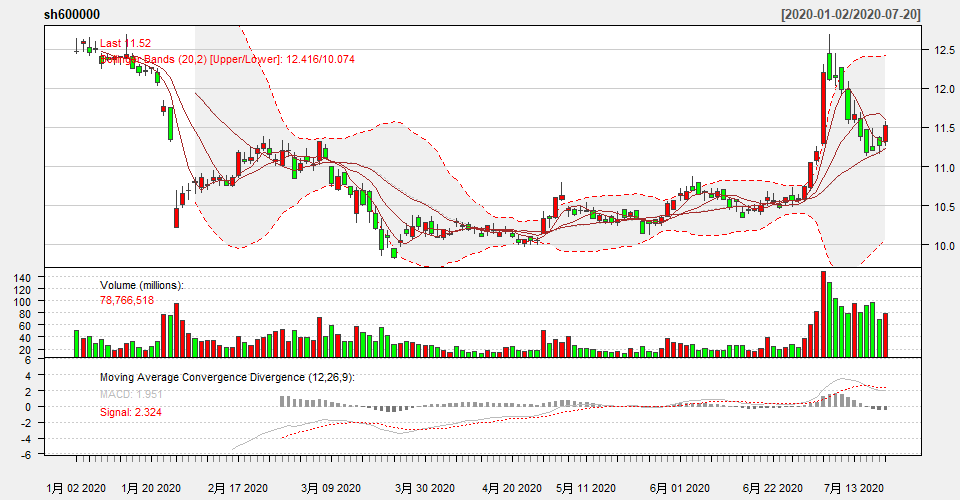
\includegraphics[width=0.95\linewidth]{figs/1}
		\caption[图1]{图形样例}
		\label{fig:1}
	\end{figure}
	

	
	
	
	
	\section{指标选择及描述}
	由于。
	
\section{模型建立}
	
	\subsection{数据处理}
	
		进行数据处理。
		
	\subsection{预测模型}
	
		正文部分。
		
		
	\subsection{模型}
		
		数量。
		
	
\section{模型求解}
	
	根据上面的模型建立过程,直接调用R中的函数求解如下:
	
	\subsection{指数模型}
	
	使用函数进行预测。
	
	\subsection{模型}
	
		针对模型。
		
		
		
		% TODO: \usepackage{graphicx} required

		
\section{结果分析}
	
	断。
	
	
\section{总结与体会}
	
	\subsection{论文总结}
	
	本文
	
	\subsection{心得体会}
	
	在。
	
	
\begin{thebibliography}{1}		
		
\bibitem{1}
R.~I.Kabacoff.
\newblock {\em R语言实战(第2版)}.
\newblock 人民邮电出版社, 2016.


\bibitem{2}
范剑青, 姚琦伟著, 陈敏译.
\newblock {\em 非线性时间序列—建模、预报及应用}.
\newblock  北京:高等教育出版社, 2005.
		
		
\bibitem{3}	
陈小玲.
\newblock {\em 基于ARIMA模型与神经网络模型的股价预测}.
\newblock 经济数学, 2017, 34(4).

\end{thebibliography}
	
	
	\section{附录}
	
	\subsection{源代码}
	
		i
	
	
	\subsection{数据包}
	
	日线
	

	
	
\end{document}